\chapter{Results}
\label{sec:ergebnisse}
This chapter explores the results obtained from simulations using greedy algorithm, considering scenarios with and without tasking. It also looks into the effects of various weighting schemes discussed in earlier chapters. The simulations produce output files named detections, tracklets, and ephemerides, 
containing essential details like detection ID, fake NORAD ID, epoch, Signal-to-Noise Ratio (SNR), orbital elements, and other relevant information. The figures and findings presented in this chapter are based on the data extracted from these output files, providing a detailed analysis of algorithmic 
performance, the impact of tasking, and the influence of different weighting schemes.\\

\section{Comparison}
To evaluate and contrast the effectiveness of the tasking algorithm and various weighting schemes, an optical telescope sensor located at the Optical Ground Station in Tenerife, Spain, was employed. The optimization involved scanning within a range of $-5$ * FOV to $+5$ * FOV for both right ascension and declination. The comparison encompassed scenarios without the use of a sensor tasking algorithm, with the implementation of the Greedy algorithm explained in a previous section, and with tasking algorithms incorporating updated cost functions based on the number of detections and time since the last detection.\\

In the initial weighting scheme, prioritizing objects based on the number of detections, Figure~\ref{fig:UniqueObj_det} shows a threshold range of 100-300 for linear weighting facilitated the detection of a new object. As seen in Figure~\ref{fig:Totdet_det} Comparing the number of detections within this scheme, slightly more were observed compared to other threshold values, signifying a noteworthy enhancement over simulations conducted without tasking.\\

\begin{figure}[H]
	\centering
	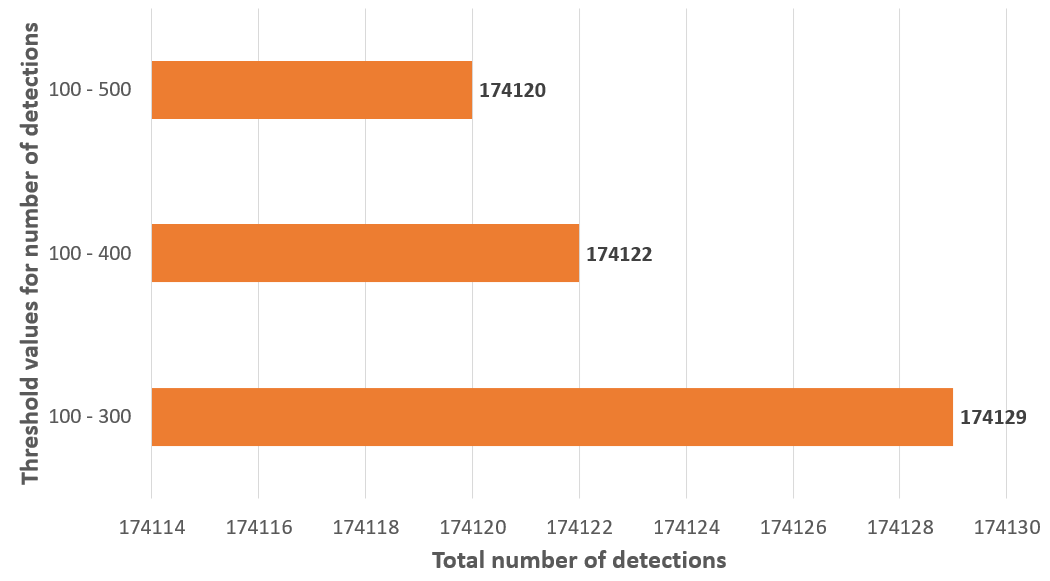
\includegraphics[width=0.8\textwidth]{Totdet_det.png}
	\caption{Total number of detections based on threshold values for number of detections of object}\label{fig:Totdet_det}
\end{figure}

\begin{figure}[h!]
	\centering
	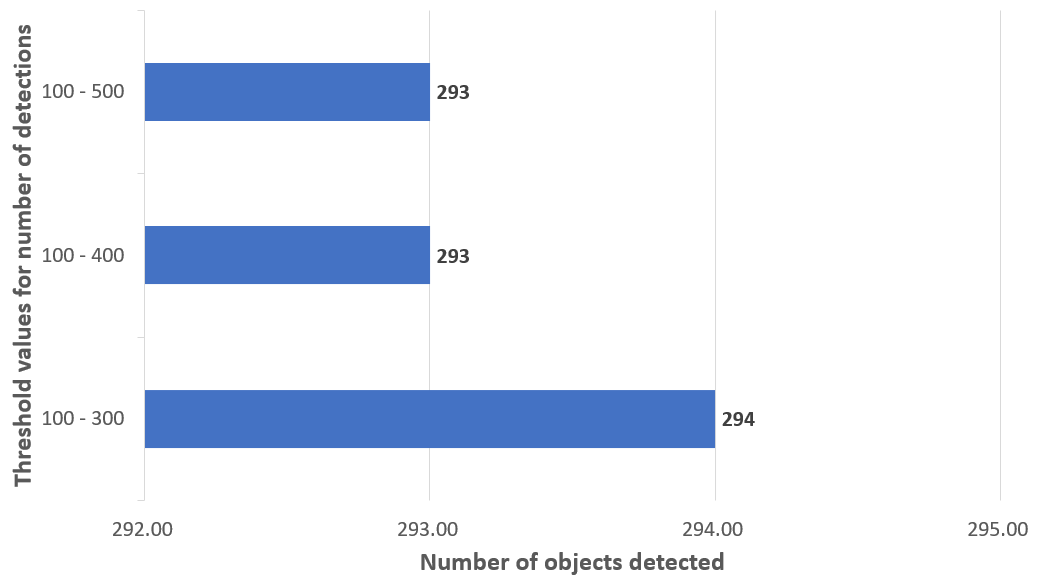
\includegraphics[width=0.8\textwidth]{UniqueObj_det.png}
	\caption{Total number of unique objects detected based on threshold values for number of detections of object}\label{fig:UniqueObj_det}
\end{figure}

Considering the second weighting scheme, which incorporates time since the last detection, among three scenarios seen in Figure~\ref{fig:Totdet_time}, the weightings within the range of 0 to 72 hours yielded the highest number of detections. However, the count of uniquely detected objects remained constant i.e. 293.\\

\begin{figure}[h!]
	\centering
	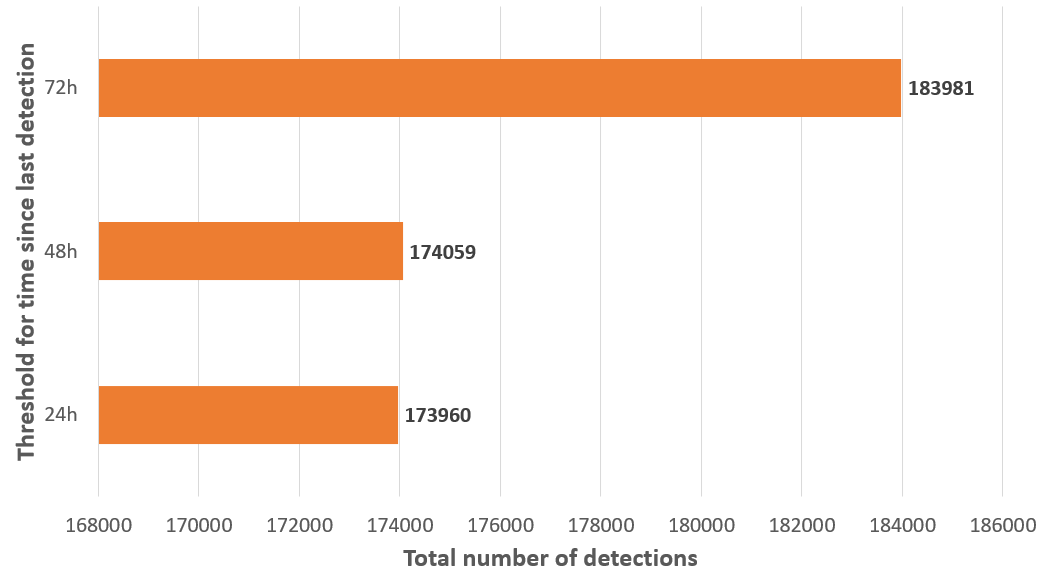
\includegraphics[width=0.8\textwidth]{Totdet_time.png}
	\caption{Total number of detections based on threshold values for time since last detection}\label{fig:Totdet_time}
\end{figure}

For the comparative analysis between scenarios without tasking and with tasking, employing combined weighting schemes, the most effective approach was selected. This involved threshold values of 100-300 and time since the last detection up to 72 hours. This selection led to a significant improvement, detecting 300 detections compared to 285 without tasking, as illustrated in Figure~\ref{fig:numbofobj}, depicting the unique objects detected in comparison to the scenario without tasking. Figure~\ref{fig:numbofdet} shows that sensor tasking with the weightings also has significantly improved the performance of number of detections compared with simulation without tasking.\\

\begin{figure}[H]
	\centering
	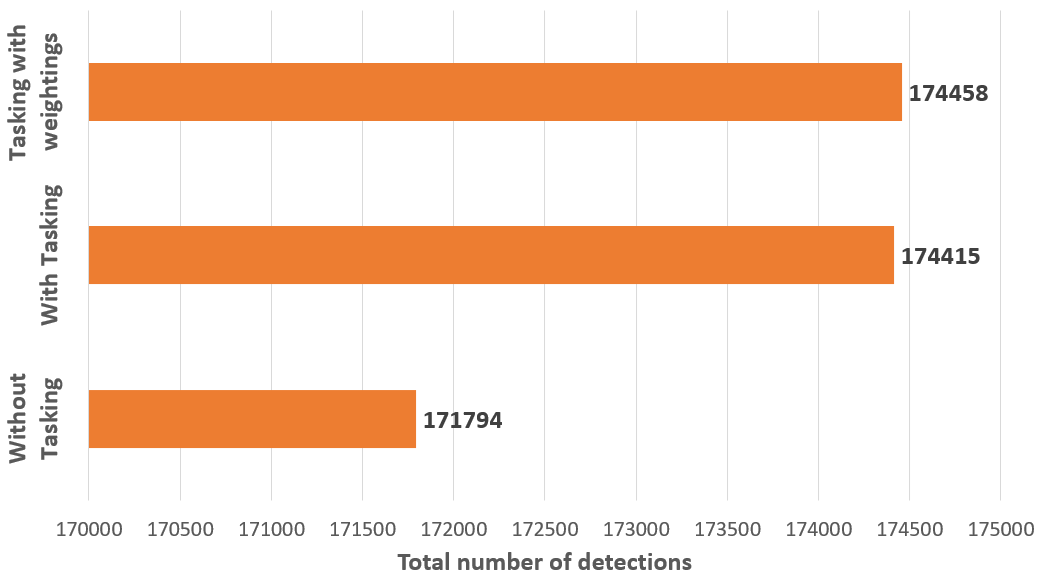
\includegraphics[width=0.8\textwidth]{numbofdet.png}
	\caption{Total number of detections compared with simulations without tasking, with tasking and tasking with Weightings}\label{fig:}\label{fig:numbofdet}
\end{figure}

\begin{figure}[h!]
	\centering
	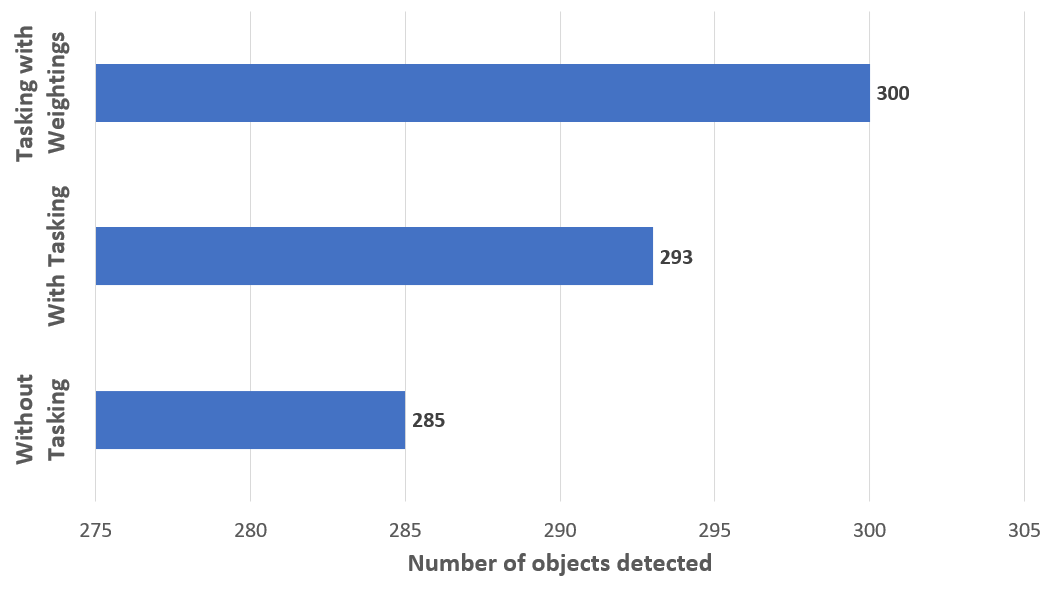
\includegraphics[width=0.8\textwidth]{numbofobj.png}
	\caption{Total number of objects compared with simulations without tasking, with tasking and tasking with Weightings}\label{fig:}\label{fig:numbofobj}
\end{figure}


\begin{figure}[H]
	\centering
	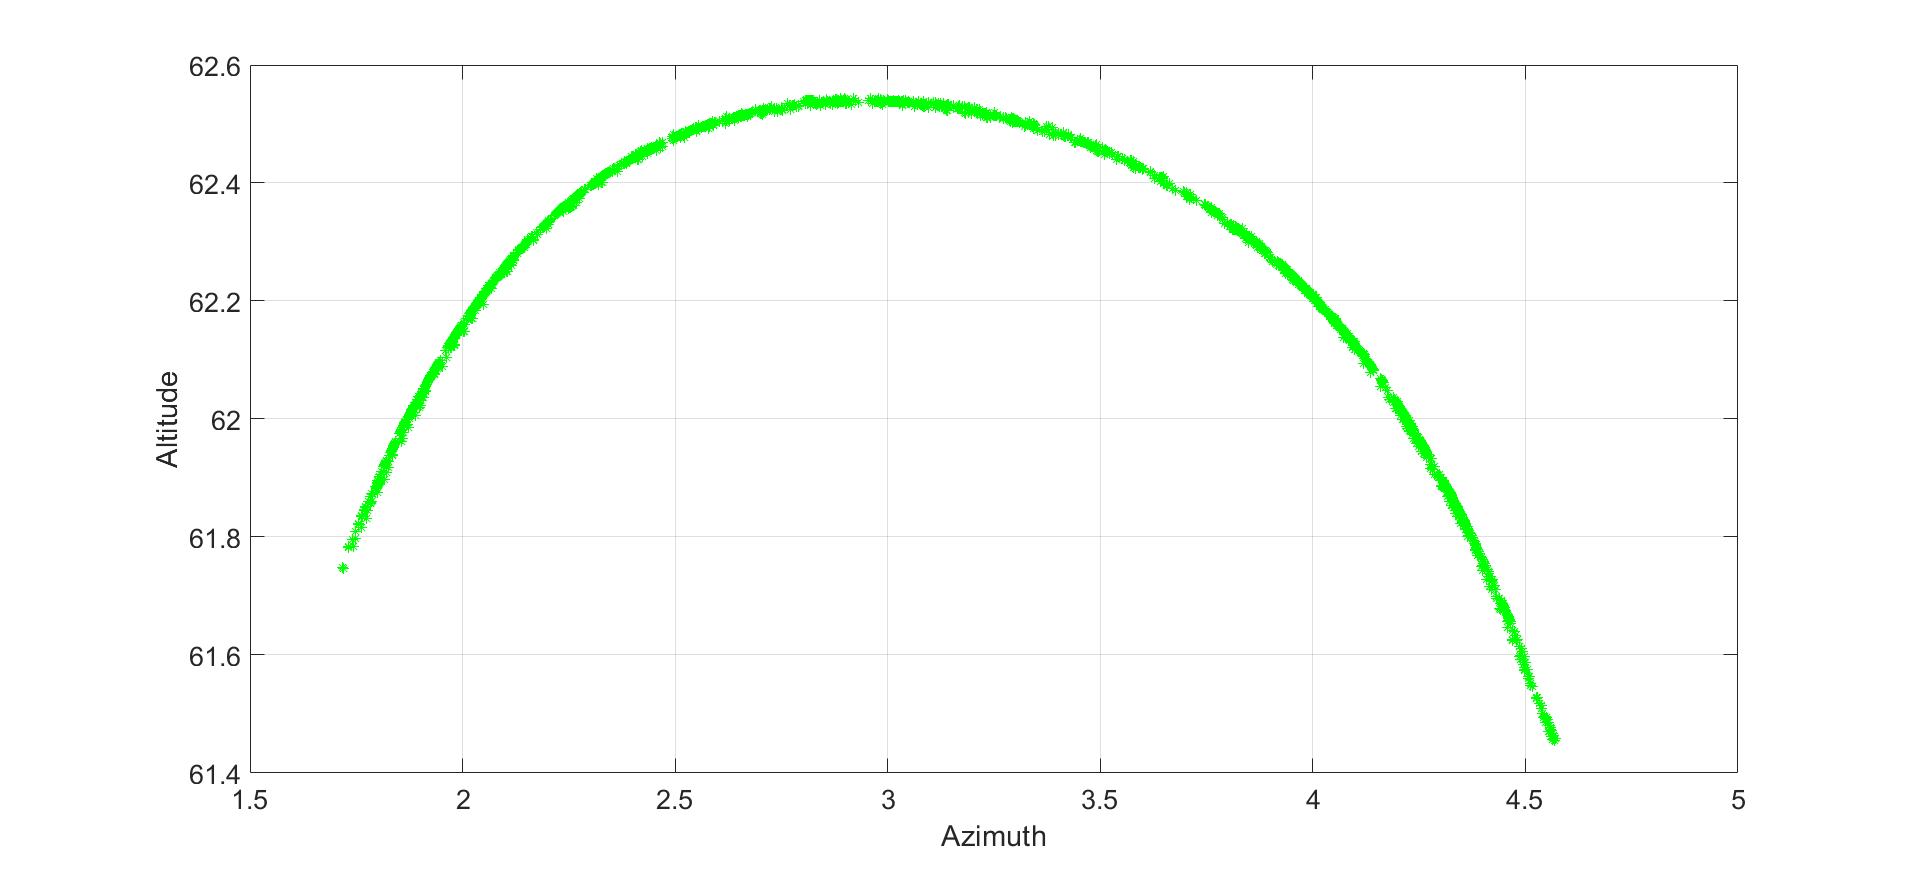
\includegraphics[width=0.9\textwidth]{AltvsAzHCS_1.png}
	\caption{Detections recorded by OGS in HCS (Without tasking)}\label{fig:}
\end{figure}


\begin{figure}[H]
	\centering
	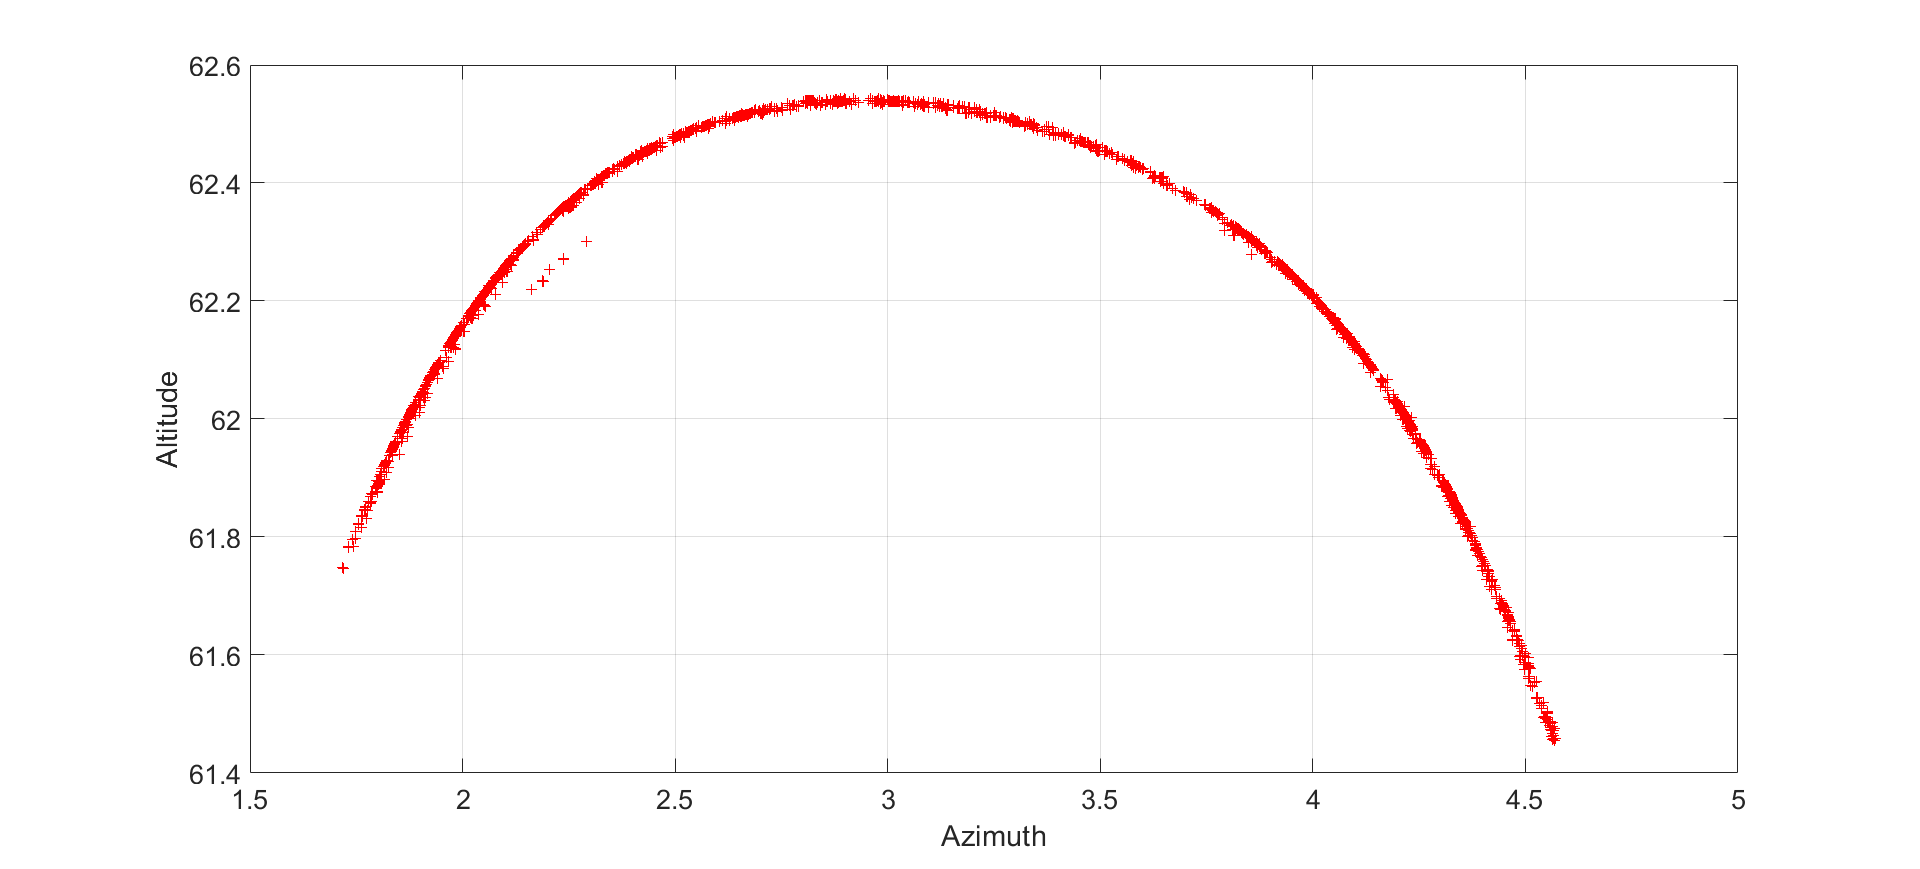
\includegraphics[width=0.9\textwidth]{AltvsAzHCS_11.png}
	\caption{Detections recorded by OGS in HCS (Tasking with Weightings)}\label{fig:}
\end{figure}

Figure~\ref{fig:AltvsAzHCS_comb} depicts the detections recorded by OGS in the horizontal coordinate system. The red crosses refer to the new detections recorded with the sensor tasking with weightings.\\


\begin{figure}[H]
	\centering
	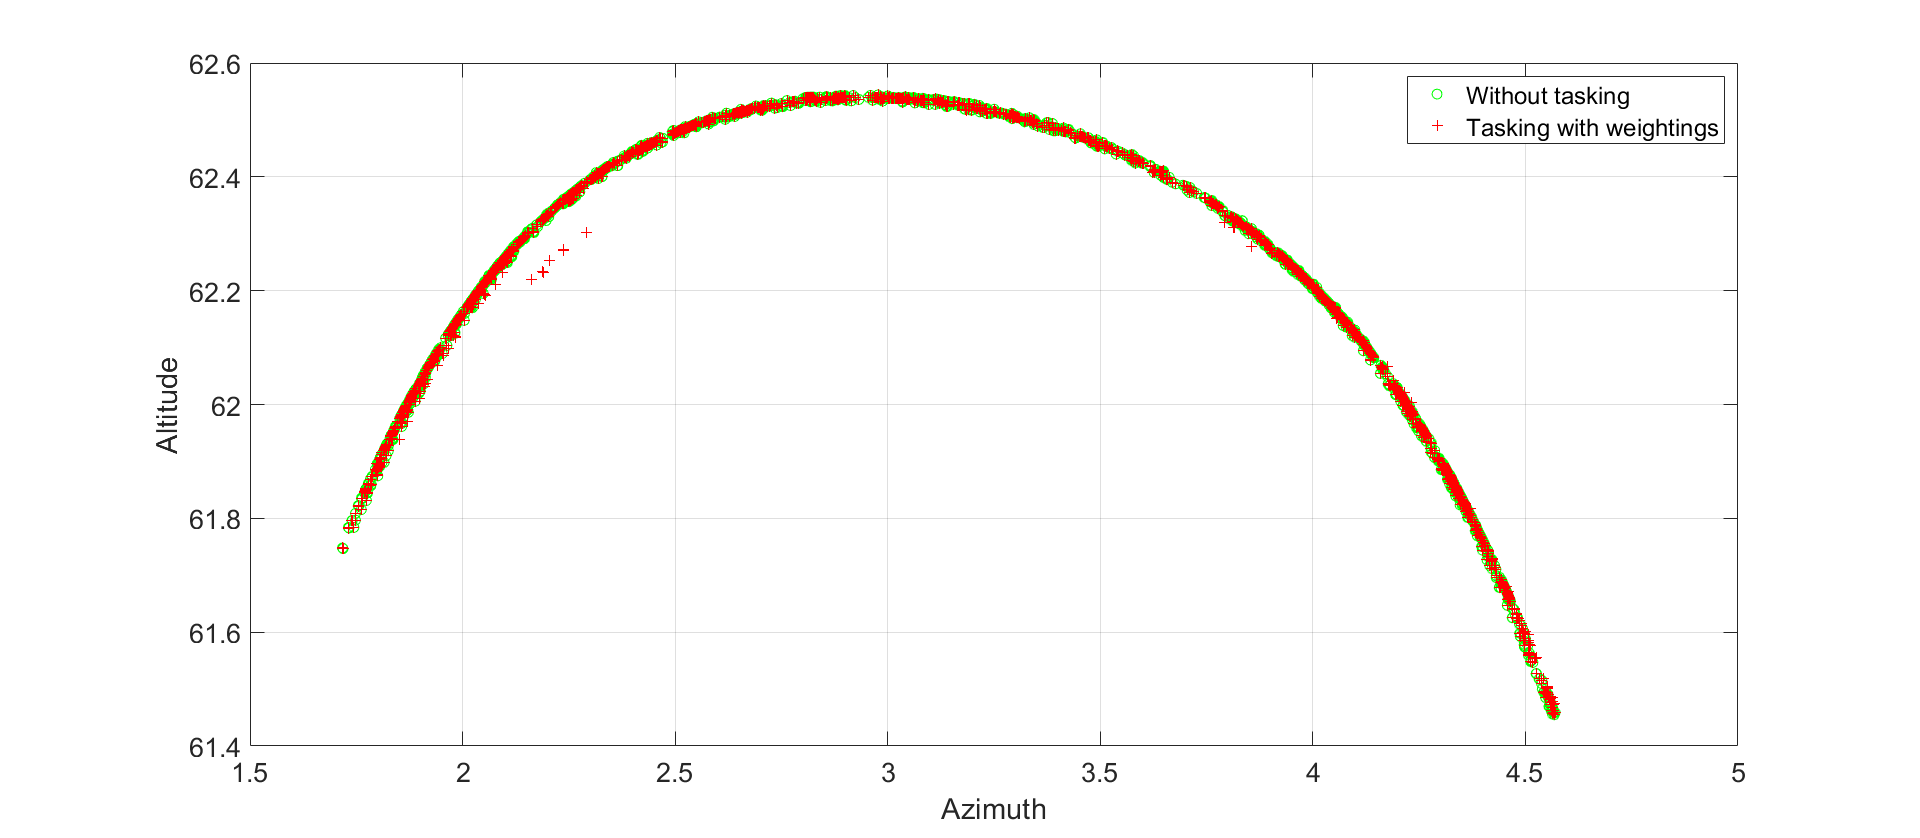
\includegraphics[width=0.95\textwidth]{AltvsAzHCS_comb.png}
	\caption{Detections recorded by OGS in HCS combined}\label{fig:AltvsAzHCS_comb}
\end{figure}


\begin{figure}[H]
	\centering
	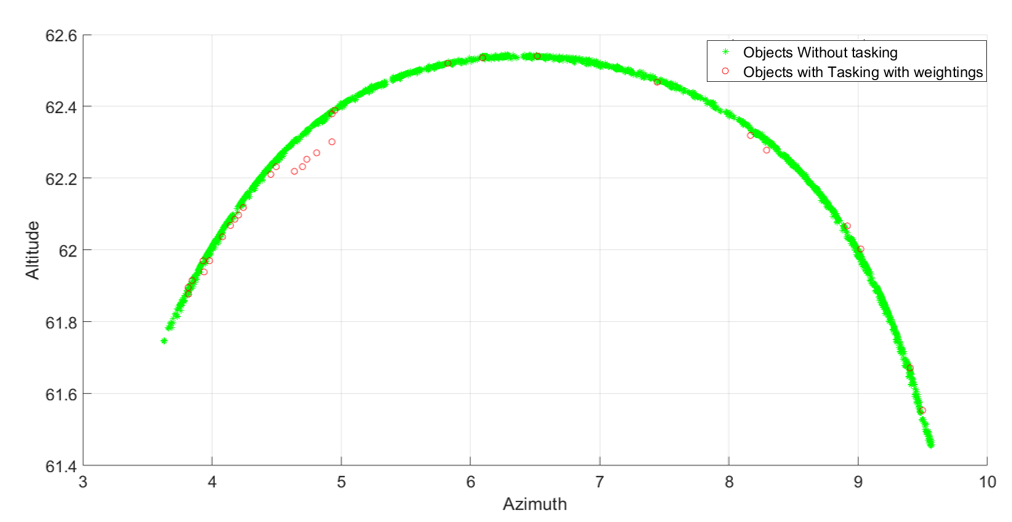
\includegraphics[width=0.95\textwidth]{AltvsAzObjects.png}
	\caption{Unique objects detected in the tasking with weightings}\label{fig:AltvsAzObjects}
\end{figure}

The employed algorithm utilized a simple stripe method for scanning the GEO vicinity, but its effectiveness in achieving an optimal search pattern is limited. Two key simplifications were introduced. Firstly, only fixed grid points in the right ascension and declination space were considered allowable viewing directions. The grid dimensions were determined by the field of view size of the sensor, ensuring comprehensive sky coverage without gaps. Improved search performance could be achieved if the spatial distribution of new targets were available, allowing the pointing direction to be set at the highest density of new targets.\\

The method's theoretical applicability extends to other orbital types besides GEO. However, careful consideration is required when designing search strategies for different orbits. Notably, a smaller grid size is sufficient for covering the GEO belt due to its dense distribution near the equator. Conversely, for different orbits like GTO and LEO, a larger field of regard might be necessary, posing challenges in discovering sparsely distributed new targets. The sensor-tasking performance is also contingent on catalog size, with surveying larger catalogs presenting computational complexities.\\
